\documentclass[letterpaper, 10 pt, conference]{ieeeconf}  % Comment this line out if you need a4paper

%\documentclass[a4paper, 10pt, conference]{ieeeconf}      % Use this line for a4 paper

%\IEEEoverridecommandlockouts                              % This command is only needed if 
                                                          % you want to use the \thanks command

\overrideIEEEmargins                                      % Needed to meet printer requirements.

\usepackage{times}
\usepackage{amsfonts}
\usepackage{amsmath}
\usepackage{bm}
\newtheorem{example}{\hspace*{-1em}\textbf{Example}}

% numbers option provides compact numerical references in the text.
\usepackage{algorithm}
\usepackage{algorithmic}

%\usepackage[]{algorithm2e}
\makeatletter
\let\NAT@parse\undefined
\makeatother

\usepackage[numbers]{natbib}
\usepackage{multicol}
\usepackage{multirow}
\usepackage[bookmarks=true]{hyperref}
\usepackage{graphicx}
\usepackage{color}
\usepackage[it,small]{caption}
\usepackage{subcaption}
\usepackage{dsfont}
\newcommand{\argmax}{\operatorname{arg\,max}}
\newcommand{\argmin}{\operatorname{arg\,min}}
\newcommand{\ve}[1]{\mathbf{#1}}

% Some illegal space-saving macros
  \parskip=3pt
  \abovedisplayskip 3.0pt plus2pt minus2pt%
 \belowdisplayskip \abovedisplayskip
\renewcommand{\baselinestretch}{0.97}



\newenvironment{packed_enum}{
\begin{enumerate}
  \setlength{\itemsep}{0pt}
  \setlength{\parskip}{0pt}
  \setlength{\parsep}{0pt}
}
{\end{enumerate}}

\newenvironment{packed_item}{
\begin{itemize}
  \setlength{\itemsep}{0pt}
  \setlength{\parskip}{0pt}
  \setlength{\parsep}{0pt}
}{\end{itemize}}


 \newlength\savedwidth
 \newcommand\whline[1]{\noalign{\global\savedwidth\arrayrulewidth
								\global\arrayrulewidth #1} %
					   \hline
					   \noalign{\global\arrayrulewidth\savedwidth}}
 \renewcommand\multirowsetup{\centering}


\newlength{\sectionReduceTop}
\newlength{\sectionReduceBot}
\newlength{\subsectionReduceTop}
\newlength{\subsectionReduceBot}
\newlength{\abstractReduceTop}
\newlength{\abstractReduceBot}
\newlength{\captionReduceTop}
\newlength{\captionReduceBot}
%\newlength{\nameReduceTop}
\newlength{\subsubsectionReduceTop}
\newlength{\subsubsectionReduceBot}

\newlength{\horSkip}
\newlength{\verSkip}

\newlength{\figureHeight}
\setlength{\figureHeight}{1.7in}

%\newlength{\figureFraction}
\setlength{\horSkip}{-.09in}
\setlength{\verSkip}{-.1in}
%\setlength{\figureFraction}{.195}


%
\setlength{\subsectionReduceTop}{-0.08in}
\setlength{\subsectionReduceBot}{-0.05in}
\setlength{\sectionReduceTop}{-0.08in}
\setlength{\sectionReduceBot}{-0.10in}
\setlength{\subsubsectionReduceTop}{-0.06in}
\setlength{\subsubsectionReduceBot}{-0.05in}
%
%
%\setlength{\figureHeight}{1.5in}
\setlength{\abstractReduceTop}{-0.15in}
\setlength{\abstractReduceBot}{-0.05in}
%
%

%\setlength{\nameReduceTop}{-0.05in}


\setlength{\captionReduceTop}{-0.09in}
\setlength{\captionReduceBot}{-0.12in}

\newcommand{\todo}[1]{\textcolor{blue}{\textbf{#1}}}

\graphicspath{ {images/} }

\pdfinfo{
   /Author (Ashesh Jain)
}


\begin{document}

% paper title
%\title{Learning Temporal Driving Models \\ for Anticipating Maneuvers }
\title{Planit dave}
 %\title{%Learning Contextual Temporal Models for Anticipating Driving Maneuvers \\ \\
%Learning Contextual Temporal Models of \\ Driving for Anticipating  Maneuvers \\ \\
%Learning Temporal Driving Models with Multi-modal Context for Anticipating Maneuvers \\
% Learning Contextual Temporal Models of \\ Driving for Anticipating  Maneuvers}

% You will get a Paper-ID when submitting a pdf file to the conference system
\author{Authors\\
Cornell University and Stanford University\\}


\maketitle
\maketitle

\IEEEpeerreviewmaketitle


\begin{abstract}

Designing systems which combine different robotic tasks (e.g., language and planning) is challenging problem. Most robotics project perform particular task and are difficult to combine and generalise across different environments , they even require different kinds of human involvement like hand crafting features and/or different feedback mechanisms.
We aim at building such a joint systems where the entire system can be improved by single weak feedback mechanism on the joint system. The feedback is given on the end-to-end system rather than the individual systems.
Experiments show that we can achieve performance close to the expert systems via much simpler feedback and using much less examples.


\end{abstract}




% !TEX root = main.tex
\section{INTRODUCTION}
Building a reliable end-to-end robotic system consisting of several modules is a challenging task.
A robot system, such as a robot that can make coffee [Jae], fold towel [], consists of several
modules such as for object recognition, path planning, language understanding, manipulation. These modules
are generally developed individually and there performance may not be optimal for the entire pipeline or they may fail due to incompatibility reasons which are hard to predict beforehand.

Previous works such as \cite{abbeel2010autonomous} have used expert feedback to recover from these failures. However, obtaining expert feedback is expensive and not always possible. In this paper, we take a co-active learning[cite] approach for an end-to-end robot system consisting of several robot modules. We particularly focus our attention on particularly two important modules namely language grounding and planning.

In a co-active learning setting, the user marginally improves the output of the system which is then used by the system for updating itself. This approach offers the advantage that user does not necessarily have to provide the optimal output. This allows the setting to work in cases where optimal output is not obvious or is expensive to obtain. 

Previous works using this approach, have looked at robot system with single modules such as [planit, tellmedave etc.] 
In this work, we expand this line of research to robot systems with multiple modules by showing how to propagate the co-active feedback given to the end observable output through the pipeline to the constituting modules.
%In a joint end-to-end system many robotic tasks fail.  \\

%Real-life systems fail, failure is expensive. Obtaining expert feedback is tough.
%Therefore crowd-sourced approaches are useful. Detailed feedback is difficult to
%give. With weak like-dislike feedback notable improvements can be shown in the
%end-to-end system.  \\

In this paper, our main contributions are two fold: we first provide a general mechanism
for using co-active feedback for complex robot systems. Secondly, we provide an empirical validation of 
our algorithm by improving a robot system for mapping natural language descriptions to navigation  trajectories. Our experiments also show that the final improved robot system, performs close to the robot system with each module trained separately using expert feedback.
%With our algorithm, we can get significant improvement in end to end system. \\

%Our experiments show that we can converge to expert feedback system and we fixed
%this particular aspect of the system.

% !TEX root = main.tex
\section{Related Work}
In this paper, we present a novel co-active learning setting for complex robot systems with application to the problem of mapping natural language descriptions to robot trajectories. This brings together three themes--- co-active learning, natural language understanding and planning trajectories.

\noindent\textbf{Co-active Learning.}

\noindent\textbf{Natural Language Understanding.} \todo{maybe add a landing line} Past decade has seen significant research in the problem natural language understanding. \cite{tellex2011understanding,fasola2013using,misra2014tell,chen2010training,artzi2013weakly,matuszek2012grounded, Mei2015Navigational,branavan2012learning} have looked at the problem of mapping natural language commands to robot actions. These works, however are chiefly concerned with parsing the commands and do not jointly model scene understanding or trajectory planing. The domain considered is either a virtual world \cite{chen2010training,artzi2013weakly,matuszek2012grounded, Mei2015Navigational,branavan2012learning} or the scene understanding and planing are performed in a sequential pipeline with the natural language understanding \cite{tellex2011understanding,misra2014tell}. Sequential modeling means that the entire pipeline may not be optimally tuned for the end to end task. 

\noindent\textbf{Trajectory Planning.}

\iffalse
The TellMeDave system translates natural language sentences to actions
sequences. PlanIt systems evaluates planning trajectories based on human
context. We have combined the systems resulting in an end-to-end system which
uses RoboBrain for features running on Weaver. 
\fi



% !TEX root = main.tex
\section{Problem Overview}

An end-to-end robotic system consists of cascade of modules which are designed to enable specific robotic abilities such as grasping, path planning, language understanding etc. In this
work we address the problem of learning such end-to-end systems in an interactive manner with a human-in-the-loop. We want the interactive learning procedure to be easy for any non-expert user to use. Such non-expert users are typically agnostic to the individual modules involved in the overall robotic system and therefore cannot manually tune each module. In fact they can at best judge the final behaviour produced by the robot. We propose an interactive procedure, where by simply observing user feedback on the final output produced by the robot, the entire robotic system can be learned.

In our formulation we consider cascade of modules that accomplish a robotic task, where the output of one module forms the input to the module following it. The input into the cascade is a robotic task description which is then forward propagated through multiple modules. The last module in the cascade generates the final robot behaviour which is visible to the user e.g. a trajectory accomplishing the task. In our learning setting, we elicit a \textit{coactive feedback} from the user on the final robot behaviour. Through this feedback the user slightly improves upon the output produced by the robot, but never reveals the optimal behaviour. Our feedback mechanism has certain desirable characteristics: (i) it is \textit{weak}, in the sense the non-expert user never reveals the optimal behaviour to the robot; and (ii) it is \textit{global}, in the sense the user does not provide feedback at the module level and only improves upon the final robot behaviour. The \textit{global} nature of feedback makes learning challenging since the user feedback needs to be propagated through each module. We now formally define the learning setting.

\section{System Overview}
System consists of an interactive web based interface where user can see the robotic tasks
executed for a particular NLP instruction. User can give their like and dislike
over this output. User can also provide a more detailed feedback whereby user stops the robot, drags it and thus updates the robot trajectory. In the present work, we work with the detailed feedback and aim to utilise the weak like dislike feedback in the future work.

\begin{figure}[h]
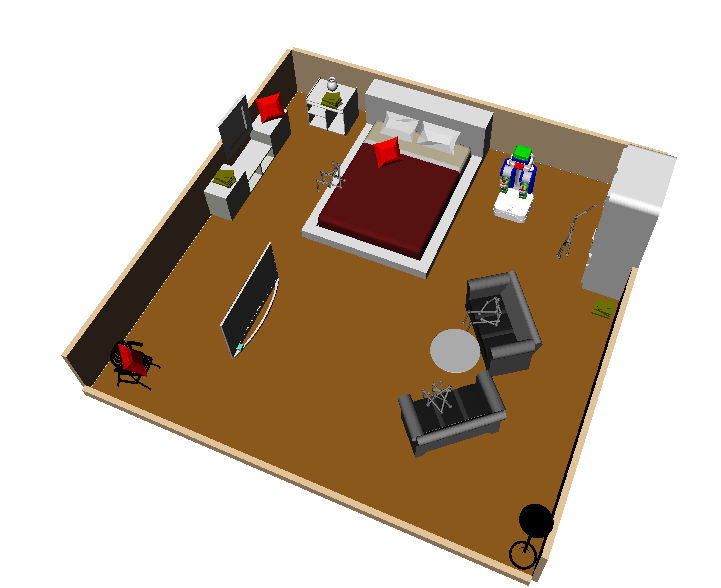
\includegraphics[width=8cm]{env}
\centering
\caption{Robotic simulator to capture user feedback}
	\label{fig:env}
\end{figure}


% !TEX root = main.tex
\section{Problem Formulation}
In this section we formally describe the learning procedure. We consider modules $M_1,M_2,...,M_N$ connected to form a cascade. Input into  module $M_i$ is denoted by $x_i$ and its output by $y_i$.  Modules are connected such that the output of $M_{i-1}$ forms the input into $M_i$, i.e. $y_{i-1} = x_i$. Each module further defines a function $f_i(x_i,y_i;\theta_i)$ jointly over its input $x_i$ and output $y_i$, and parametrized by $\theta_i$. The input into the cascade is task $x_1$, and the output robot behaviour presented to the user is $y_N$. 	We further assume a function $U(x_{i},y_{i})$ which conveys how much the user values output $y_{i}$ for input $x_{i}$ at a particular module $i$. We further assume a function $U(x_1,y_N)$ which conveys the performance of the entire system, though such a function is never observed. The algorithm only gets to observe user feedback on $y_N$ and none of the $y_{i}$'s are known. We have designed a heuristic that maps the output $y_{N}$ to the output sequence $y_{i}$ for different modules and learn their parameters. Our learning setting iteratively performs the following steps:
\begin{enumerate}
\item At each iteration $t$, the robot is presented with a task $x_1$ and it generates behaviour $y_{N,t}$ which is presented to the user
\item The user provides a feedback $\bar{y}_{N,t}$ by improving upon ${y}_{N,t}$ such that $U(x_1,\bar{y}_{N,t}) > U(x_1,{y}_{N,t})$
\item Heuristic maps the feedback $y_{N}$ to the sequence of output $\bar{y}_{1}, \bar{y}_{2} \dots \bar{y}_{N-1}$ for different modules
\item The parameters $\{\theta_1,...,\theta_N\}$ of the entire cascade are updated using the utility functions $U(x_{i},y_{i})$ and the mapped output
\end{enumerate} 

The learning setting with the designed heuristic described above extends coactive learning~\citep{Jain13,Shivaswamy12} to a system with multiple modules and a single feedback. Upon receiving the user feedback, parameters of module $M_i$ are updated using the following perceptron equation:  
\begin{align}
\theta_i \leftarrow \theta_i +  \frac{\partial U_i(x_i,\bar{y}_i)}{\partial \theta_i} &- \frac{\partial U_i(x_i,{y}_i)}{\partial \theta_i}
\end{align}
% In the above equations the	 gradient $\frac{\partial f_N(x_N,\bar{y}_N)}{\partial \theta_i}$ is calculated using backpropagation as follows:
% \begin{align}
% \frac{\partial f_N(x_N,\bar{y}_N)}{\partial \theta_i} &= \frac{\partial y_i}{\partial \theta_i}  \frac{\partial f_N(x_N,\bar{y}_N)	}{\partial y_{i}}\\
% \frac{\partial f_N(x_N,\bar{y}_N)	}{\partial y_{i}} &= \frac{\partial y_{i+1}	}{\partial y_{i}} \frac{\partial f_N(x_N,\bar{y}_N)	}{\partial y_{i+1}}
% \end{align}
By mapping the feedback to different modules of the cascade using the designed heuristic, we incorporate the corrective user feedback to update each module in the cascade. The progress made by the learning algorithm is measured by its regret which is given by the following equation:%~\eqref{eq:regret} which cannot be directly observed.
\begin{equation}
\label{eq:regret}
REG_T = \frac{1}{T}\sum_{t=1}^T U(x_{1,t},y_{N,t}^*) - U(x_{1,t},y_{N,t}) 
\end{equation}
Here $y_{N,t}^*$ is the optimal robot behaviour for $x_{1,t}$, and $y_{N,t}$ is the behaviour predicted by the algorithm at iteration $t$. The regret cannot be directly observed as $y_{N,t}^*$ and utility $U$ are not observable. However, if the user at each iteration incrementally improves upon $y_N$ then the regret asymptotically decays to zero under mild constraints~\citep{Shivaswamy12,Jain13}.  

% !TEX root = main.tex
\section{Experiments}
\subsection{Dataset}
Our dataset consists of 90 natural language instructions of which 60 are a sequence of simple move to instructions and 30 are high level natural language instructions. All these instructions are taken using a \href{http://52.25.65.189:9000/#/getFeedback}{crowd sourcing system} and the ground truth for the natural language instructions are also collected for evaluating the model. The instructions are taken for 16 different environments depicting scenes similar to living room, bedroom and kitchen. \\
The environments are constructed in OpenRAVE with context generated from 6 different human activities depicted by skeletals. The activities considered are walking, watching, interacting, reaching, sitting and working. \\
The instructions involve task description for themes in common house-hold enviromnent like cleaning the room, arranging the guest room and serving coffee and also some simple instructions like move to the bed and then to the table. The dataset contains considerable high level ambiguous instructions like distribute, arrange etc. with variety in verbs.\\
The dataset was divided into 60-30 ratio for training and testing purposes respectively.  

% Please see supplementary for examples from our dataset.

\subsection{Set Up:}
	\subsubsection{Planit with Coactive Feedback:} 
		Planit is a crowd source platform that captures human interaction with the environment and learn their preferences over trajectories. Earlier version of planit was trained using expectation maximization using a database of 2500 trajectories over 112 different environments. In the current setting, we aim to to learn user preferences via coactive learning which requires a sub optimal feedback from the user which is more flexible to obtain and requires fewer number of training examples.

		Dataset consists of 16 different environments with 5 different activities occuring in them namely watching, walking, reaching, interacting, etc. User can view the environment in a simulator and can drag the robot to different positions in the environment. User provided the feedback in the form of a pair ($y,\bar{y}$) whereby $U(y) < U(\bar{y})$. This implies that the robot position $\bar{y}$ is more favourable for the user than the robot position $y$ in any trajectory in the environment. 

		Total 432 feedback was collected from the user across 10 different environment. For evaluation, we considered a set of 6 environments (not in the training set) from the dataset. The trained model was used to rank 112 trajectory sets each containing 7 trajectories to move between two randomly sampled points $A$ and $B$. Original version of planit (as reported in the planit paper (expert system) was assumed as the ground truth for evaluating the trajectories. The nDCG (normalized discounted cumulative gain) of \textbf{0.89} for the above model was observed. This is reasonable since in the earlier version the feedback was expert (labelling segments of 2500 different trajectories) and in the given system we have 400 instances of much weaker feedback.\ref{fig:planitResult} 


		
		% 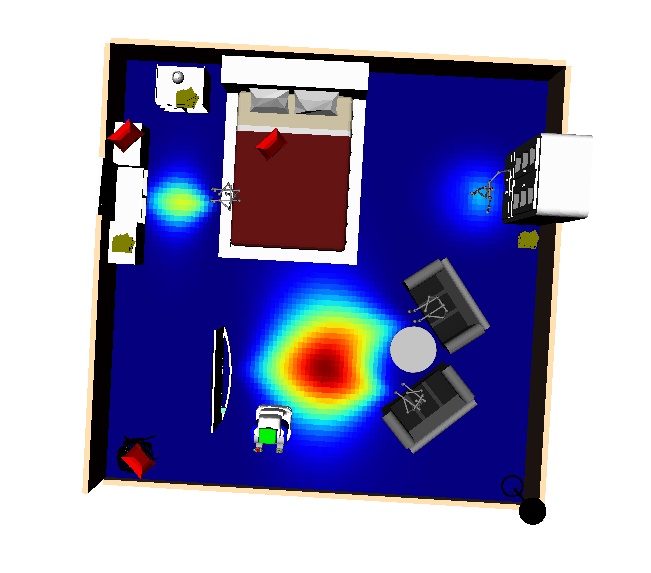
\includegraphics[scale=0.5]{planitResult}
		\begin{figure}[h]
		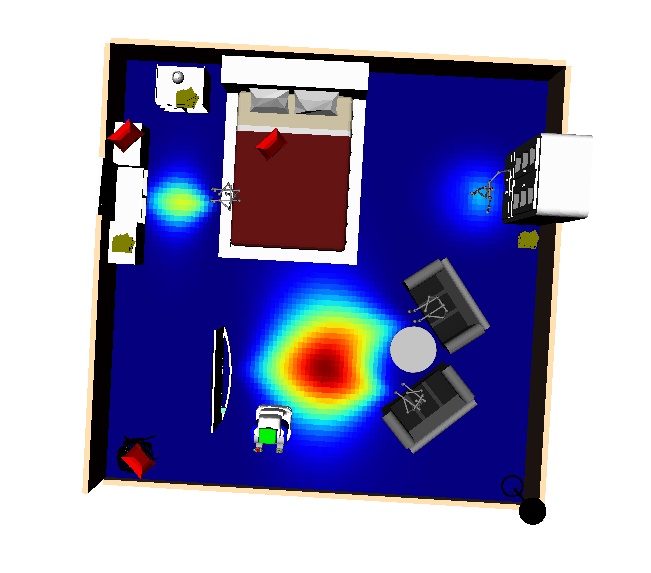
\includegraphics[width=8cm]{planitResult}
		\centering
		\caption{Cost function learnt via Coactive Feedback}
  		\label{fig:planitResult}
		\end{figure}


		\begin{figure}[h]
		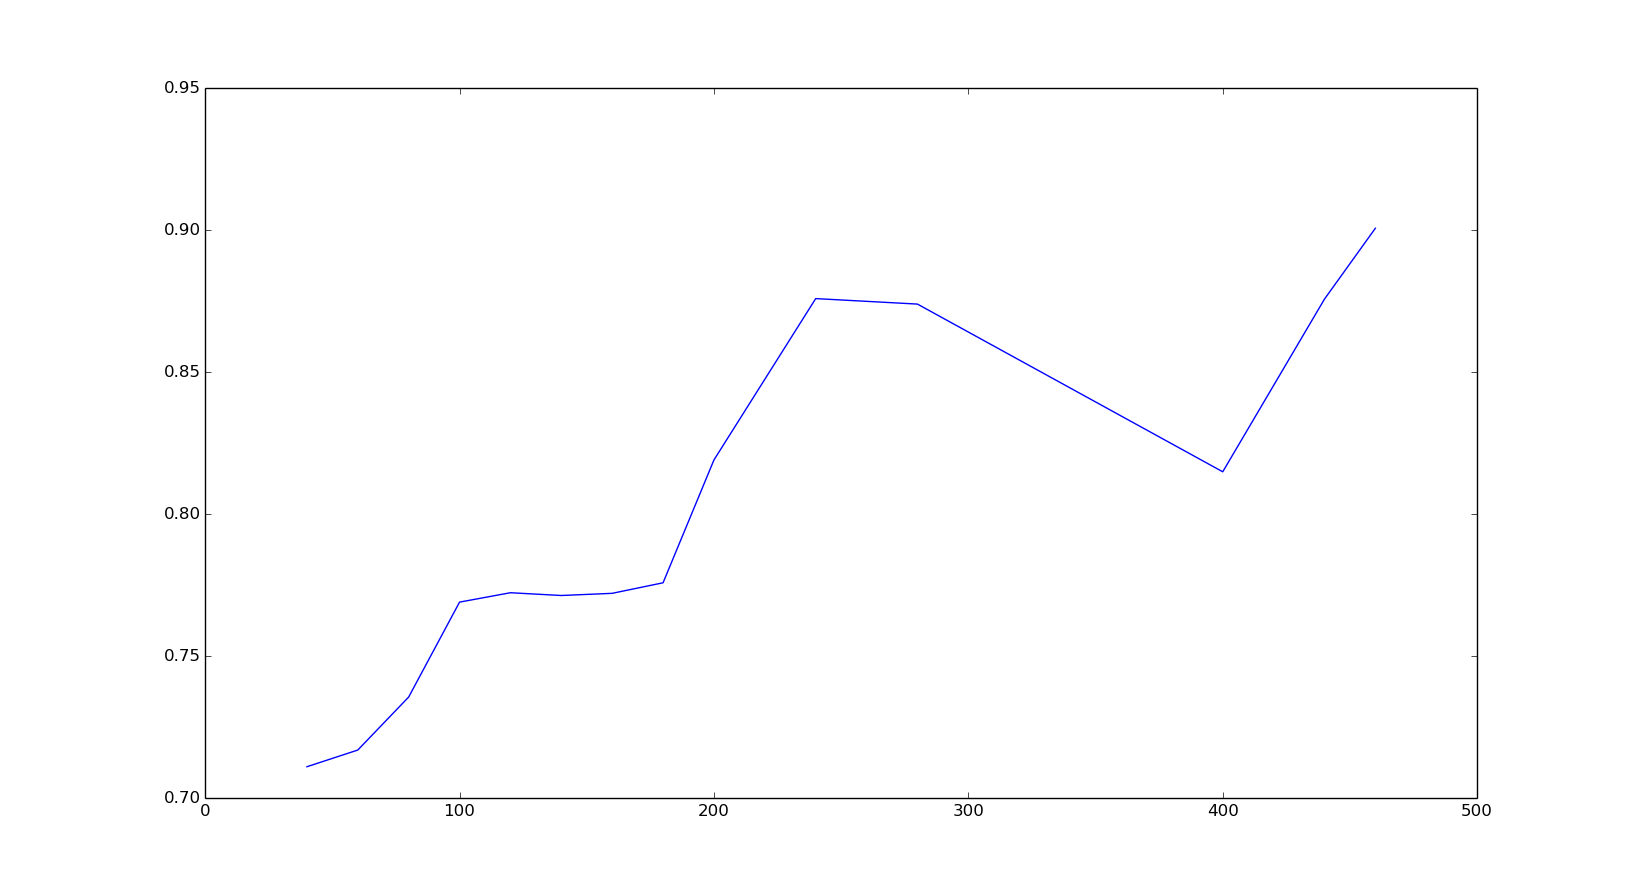
\includegraphics[width=9.5cm]{coactiveVSfeed}
		\centering
		\caption{Coactive Learning aginst number of feedbacks}
  		\label{fig:c1}
		\end{figure}
	\subsubsection{TellMeDave with Coactive Feedback:} 
	TellMeDave is system that grounds Natural Language instructions to sequence of robotic actions by capturing the context from the environment. The original version of Tellmedave was trained with stochastic gradient descent over 4 tasks performed in 5 different environments with 50 NL instructions on each. \\
	As mentioned earlier, we aim to to learn user preferences via coactive learning which requires a sub optimal feedback from the user. Dataset chosen was same as that mentioned in the Dataset section with 60 train points and 30 test points containing high-level and low-level NL desciptions of the tasks. \\
	The end-user gave feedback on each of the datapoints from the training set in the form of detailed descriptions. This feedback was hard to get due to difficulty in detecting the error in the pipeline i.e. whether the mistake lies in lexicon selection or object selection. \\
	Evaluation Metrics. We consider two metrics, IED and END\cite{Misra2014tell}, which measure accuracy based on the action sequence and environment, respectively. The Instruction Edit Distance(IED)\ref{fig:IED} metric improved from 9.98\% to 30.21\% and Environment Edit Distance(END)\ref{fig:END} metric improved from 3.79 \% to 27.09\%.
 
	\begin{figure}[h]
		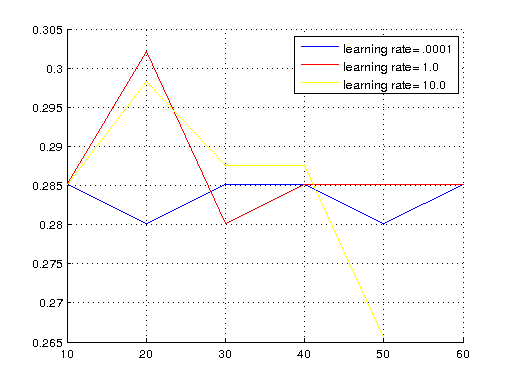
\includegraphics[width=8cm]{IED}
		\centering
		\caption{IED against different number of feedbacks }
  		\label{fig:IED}
		\end{figure}
		
	\begin{figure}[h]
		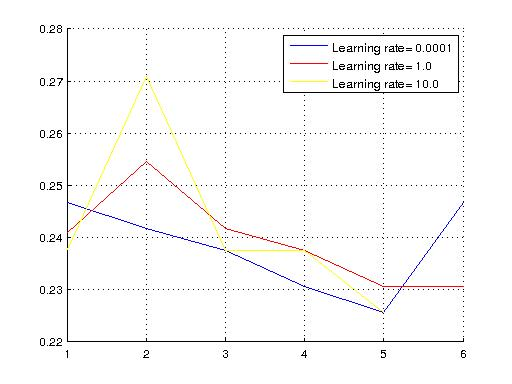
\includegraphics[width=8cm]{END}
		\centering
		\caption{END against different number of feedbacks }
  		\label{fig:END}
		\end{figure}

	\subsubsection{Joint system Coactive Feedback:}
	In the given setting we cascade the modules corresponding to the language and trajectory planing in such a way that the robot executes a sequence of instructions to perform a task specified by the natural language instruction. The dataset consists of 90 language instructions across 16 environments of which 60 were used for training and 30 were used for evaluation.

	User are shown trajectories for executing a sequence of instruction in a simulator and the user can stop trajectories and update specific waypoints of the trajectory by dragging the waypoint to a better point thus modifying the entire trajectory for performing the task.

	Thus, for a natural language instruction $x$, user observes trajectory $y$ and provides a slighly improved trajectory $\bar{y}$ for executing the instruction. Such feedback may either correspond to modification in the sequence of instructions output by the language module or updating the trajectory as per user preferences. The feedback is such that ($x,\bar{y}$) captures the intent of the user in a better way than ($x,y$).

	We have devised a heuristic that distributes the given feedback to planit and tellmedave and finds sequence of robot instructions that are consistent with the given trajectory.

	The modified trajectories on these 60 datapoints generated around 50 feedback for tellmedave and around 250 feedback for planit.(multiple waypoints can be obtained from a single trajectory improvement for learning planning parameters).

	The performance of planit was evaluated in a similar fashion as the standalone system by ranking 112 trajectory set each consisting of 7 trajectories.The nDCG (normalized discounted cumulative gain) of around \textbf{0.79} was obtained with respect to the ground truth.




\subsection{Results} %\todo{Dip: please take a detailed pass over this subsection}
We test our algorithm on two tasks, in the first task we evaluate the success of co-active feedback in tuning the robot system and in second task, we evaluate the results from different type of feedback.

\noindent\textit{Task 1: Improvement Due to Co-active feedback}
\textit{Conclusion:} The system is able to improve its accuracy by BLAH on a held-out test set, after a few iterations of co-active feebacks from non-expert users.

\begin{table}
\label{tbl:tsk1}
\caption{Table 1: System improves its end-to-end accuracy after receiving co-active feedback on the final robot behavior}
\centering
\begin{tabular}{|l|l|}
\hline
\textit{System} & \textit{Accuracy} \\
\hline
Sys & BLAH \\
Sys + CF & BLAH \\
Sys + MCF & BLAH \\
\hline
\end{tabular}
\end{table}

\noindent\textit{Task 2: Effects of Different Type of Feedback}
\textit{Conclusion:} Our system based on co-active feedback is able to achieve close performance with system using expert feedback. Further, our system vastly outperforms system based on boolean feedback.

\begin{table}
\label{tbl:tsk2}
\caption{Table 2: Co-active feedback achieves close to the performance with expert feedback}
\centering
\begin{tabular}{|l|l|}
\hline
\textit{System} & \textit{Accuracy} \\
\hline
Sys + boolean & --\\
Sys + CF & -- \\
Sys + Expert & -- \\
\hline
\end{tabular}
\end{table}


%\todo{Dip: we should also experiment with individually tuning the two system AND experiment with different number of feedback until an asymptote is attained}





\section{CONCLUSIONS}

A conclusion section is not required. Although a conclusion may review the main
points of the paper, do not replicate the abstract as the conclusion. A
conclusion might elaborate on the importance of the work or suggest applications
and extensions. 



{
\bibliographystyle{plainnat}
\bibliography{../COMTools/shortstrings,../COMTools/references}
}

\end{document}
